\capitulo{3}{Conceptos teóricos}




\section{Introducción}
Han pasado algunos años desde que se empezaron a utilizar los videojuegos como entorno de prueba para agentes inteligentes, y es que los videojuegos son un excelente campo de prueba para algoritmos de inteligencia artificial. Los videojuegos nos proporcionan un entorno controlado y predecible, lo que nos permite determinar con mayor eficacia la calidad del algoritmo. Para una mejor comprensión del trabajo realizado a continuación se exponen brevemente algunos conceptos relevantes.

\section{Minería de datos}
Vivimos rodeados de datos, cada vez que utilizamos nuestro smartphone para consultar el tiempo, realizamos un pago con tarjeta, tuiteamos... dejamos un rastro de datos. Esto es aplicable, no solo al ámbito privado, sino que es aplicable a cualquier ámbito de la industria, ya que allá donde exista un proceso, van a existir datos. Siempre se ha intuido que esa información podría resultar interesante, pero no ha sido hasta hace relativamente poco, gracias a los grandes avances en la computación, cuando hemos empezado a sacarle provecho, y sí, todo ese reguero de datos que dejamos ha resultado realmente valioso.

La minería de datos consiste en aplicar a esa gran cantidad de datos desorganizados de los que disponemos, una serie de métodos matemáticos que nos permitan transformarlos en información. Cuando hablamos de transformar datos en información, hablamos que que la minería de datos nos va a permitir extraer patrones que una persona a simple vista no sería capaz de descubrir. 

\section{Inteligencia Artificial}
La inteligencia artificial (IA) es una ciencia en auge en las últimas décadas gracias al vertiginoso crecimiento del rendimiento en el campo de la computación. En realidad no hay una única definición para IA, ya que históricamente se le han dado diferentes enfoques,siendo aplicada a diferentes campos con diversos propósitos. Russel y Norvig \cite{Russell_Norvig} sintetizan en su libro las definiciones de diversos autores con cuatro enfoques diferentes.

\begin{table}[h]
\centering
\resizebox{\textwidth}{!}{%
\begin{tabular}{|l|l|}
\hline
\multicolumn{1}{|c|}{Sistemas que piensan como humanos} & \multicolumn{1}{c|}{Sistemas que piensan racionalmente} \\ \hline
\begin{tabular}[c]{@{}l@{}}«{[}La automatización de{]} actividades que vinculamos\\ con procesos de pensamiento humano, actividades \\ como la toma  de definiciones, resolución de problemas,\\ aprendizaje...(Bellman, 1978)\end{tabular} & \begin{tabular}[c]{@{}l@{}}«El estudio de las facultades mentales mediante\\ el uso de modelos computacionales». (Charniak\\ y McDermott, 1985)\\«El estudio de los cáculos que hacen posible per-\\ cibir, razonar y actuar!.(Winston, 1992)\end{tabular} \\ \hline
\multicolumn{1}{|c|}{Sistemas que actúan como humanos} & \multicolumn{1}{c|}{Sistemas que actúan racionalmente} \\ \hline
\begin{tabular}[c]{@{}l@{}}«El arte de desarrollar máquinas con capacidad para\\ realizar funciones que cuando son realizadas por per-\\ sonas requieren inteligencia». (Kurzweil, 1990)\\ «El estudio de cómo lograr que los computadores rea-\\ licen tareas que, por el momento, los humanos hacen\\ mejor». (Rich y Knight, 1991)\end{tabular} & \begin{tabular}[c]{@{}l@{}}»La Inteligencia computacional es el estudio del\\ diseño de agentes inteligentes».(Poole et al.1998)\\ \\ «IA... Está relacionada con conductas inteligentes\\ en artefacto''. (Nilson, 1998)\end{tabular} \\ \hline
\end{tabular}%
}
\caption{Definiciones de inteligencia artificial}
\end{table}

Para el caso que nos ocupa la que más me gusta es «El estudio de cómo lograr que los computadores realicen tareas que, por el momento, los humanos hacen mejor», ya que mediante las técnicas de aprendizaje que emplearé, nos debería costar diferenciar si es un humano o una máquina quien realiza las tareas.

\subsection{Sistemas inteligentes}
 En 1995 comienzan a aparecer los sistemas inteligentes \cite{wiki:Agente_Inteligente}. Un agente inteligente es una entidad capaz de recibir estímulos de su entorno, procesar esta información y actuar en consecuencia de manera racional, maximizando la eficacia del resultado esperado.


\section{Aprendizaje Máquina}

El concepto de aprendizaje máquina, o Machine Learning, se basa en la idea de utilizar una serie de estímulos o percepciones, no sólo para la toma de decisiones, sino para mejorar la respuesta y que estas decisiones sean más certeras. Hay múltiples formas de aprendizaje que podemos clasificar en tres grupos mas amplios: aprendizaje supervisado, aprendizaje no supervisado y aprendizaje por refuerzo.


\subsection{Aprendizaje supervisado}

El aprendizaje supervisado se basa en la idea de aprender a partir de ejemplos o instancias, es decir, se le proporcionarán una serie de entradas (atributos), y sus correspondientes salidas esperadas.

\begin{table}[h]
\centering
\begin{tabular}{|c|c|}
\hline
\rowcolor[HTML]{C0C0C0} 
Entrada & Salida \\ \hline
1       & 2      \\ \hline
2       & 4      \\ \hline
3       & 6      \\ \hline
4       & 8     \\ \hline
5       & 10     \\ \hline
\end{tabular}
\caption{Ejemplo de instancias de aprendizaje supervisado}
\label{aprendizaje_supervidado}
\end{table}

En el ejemplo podemos ver un set de datos muy elemental que nos permitirá entender el aprendizaje supervisado. La entradas, o la entrada, es un único valor numérico y la salida otro valor numérico. La función que permite obtener la variable dependiente $y$ a partir de la independiente $x$ a simple vista se deduce que es: $y = 2x$. Podemos entrenar un modelo para generalizar cualquier valor mediante una sencilla regresión lineal.

\begin{figure}[h]
  \centering
    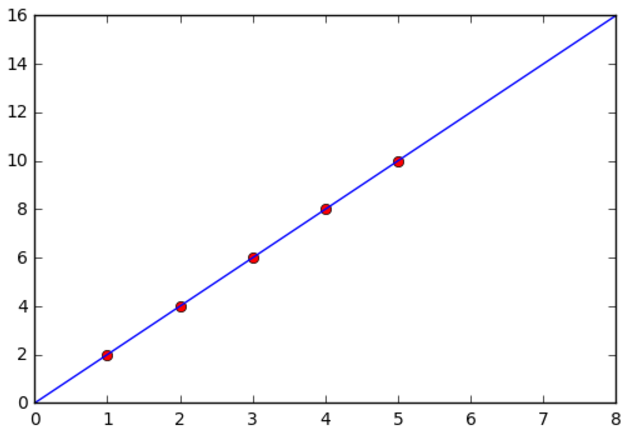
\includegraphics[width=0.5\textwidth]{../img/supervisado_grafica_1}
  \caption{Representación de la regresión lineal}
  \label{regresion_lineal}
\end{figure}

La regresión lineal permite ajustar una función a los valores proporcionados, es decir, gráficamente se debe poder trazar una línea que se encuentre a la menor distancia posible de todos los puntos. En la figura 3.1 se pueden ver en rojo los puntos que representan los valores en entrada en el eje $x$, y los valores de salida en el eje $y$, y en color azul la representación de la función, en este caso, $y = 2x$.

Llegados a este punto podríamos decir que ya tenemos un modelo «entrenado», puesto que si queremos predecir la salida que obtendríamos en, por ejemplo, $x=6$, el modelo nos devolvería el valor 12.

En este ejemplo se ha utilizado una regresión lineal. Este modelo en ciertos casos se queda corto, pero hay otros modelos de aprendizaje supervisado muy conocidos que nos permitirán hacer mejores estimaciones. En la realización de este proyecto se ha empleado una combinación de varios de estos y otros modelos, a mencionar, Decision tree (arboles de decisión), Random Forest(una variante de los arboles de decisión), MLP (perceptrón multicapa) y una red neuronal convolucional.

\subsection{Aprendizaje no supervisado}
En contraposición al aprendizaje supervisado, tenemos el aprendizaje no supervisado. En el aprendizaje no supervisado no vamos a proporcionar una salida determinada, simplemente se le proporcionan unas entradas y se espera que consiga generalizar exclusivamente a partir de los datos. La idea básica de este tipo de aprendizaje es buscar patrones en las agrupaciones de datos. Normalmente es un tipo de entrenamiento que lleva mucho más tiempo. No se profundiza más en este caso, ya que no es relevante en este proyecto.

\subsection{Aprendizaje por refuerzo}

En este tercer tipo de aprendizaje no seremos nosotros los que le indiquemos cuál es la respuesta correcta. En este tipo de aprendizaje es el propio agente el que va a aprender a partir de una serie de refuerzos o recompensas. En este caso se toma una decisión y se observa la respuesta, si esta es favorable, se ajustará la función. 

En el caso de mi proyecto, se podría hablar de una aproximación a este tipo de aprendizaje, sin tratarse exactamente del mismo. En el caso de mi algoritmo de entrenamiento, se utiliza una red neuronal cuya función de \emph{fitness} es la puntuación obtenida. Se asemeja al aprendizaje por refuerzo en el aspecto de que para mejorar la velocidad de aprendizaje, e independientemente de la puntuación del jugador, se aplicarán de forma arbitraria recompensas (para un refuerzo positivo) y penalizaciones (para un refuerzo negativo). En mi caso, el refuerzo positivo es sumar a la puntuación final el tiempo que ha estado jugando sin morir. En el caso del refuerzo negativo, aplicaremos una penalización al morir.


\section{Árboles de decisión}
Los árboles de decisión son un tipo de clasificador basados en instancias, es decir, estaríamos hablando de aprendizaje supervisado. La instancias las conforman una serie de atributos de entrada y unas clases, salidas esperadas. Dadas estas instancias, el clasificador genera una estructura de árbol en base a éstas.


\imagen{decisionTree}{Ejemplo Árbol de decisión}



\section{Redes Neuronales}
Las redes neuronales artificiales son una de las ramas de la computación de las denominadas «Bio-inspiradas'', es decir, tratan de emular de algún modo alguna de las características propias de los seres vivos. Muchos de los seres vivos precisan de neuronas para poder llevar a cabo sus actividades motoras. Una neurona es un tipo de célula cuya función es transmitir impulsos al sistema nervioso \cite{wiki:neurona}. En nuestro caso tendremos una representación digital de estos impulsos. Las neuronas de una red neuronal, al igual que ocurre en la naturaleza, se van activar conjuntamente  de forma que, neuronas que se activan conjuntamente con mucha frecuencia, refuercen sus uniones para que, cuando se tengan que volver a activar a causa de un estímulo externo, lo vuelvan a hacer conjuntamente. Este proceso de reforzar (y debilitar) las uniones es lo que se conoce como aprendizaje.


A rasgos generales las redes neuronales realizan dos tipos de funciones:
\begin{itemize}
    \item Clasificación: En la clasificación el agente inteligente que implementa la red neuronal ha de devolver una de las salidas ya especificadas anteriormente. Lo que es lo mismo, «Clasificar'' nuestros datos de entrada en uno de los grupos esperados.
    \item Regresión: En este caso nos va a devolver un valor numérico que se ajusta a una función continua, por este motivo a la regresión lineal también se la denomina ajuste de funciones.
\end{itemize}


\subsection{Perceptrón}
El modelo más simple que podemos encontrar es el perceptrón. El perceptrón es un modelo neuronal de una sola neurona con una única salida \cite{wiki:perceptron}.
\begin{figure}[]
  \centering
  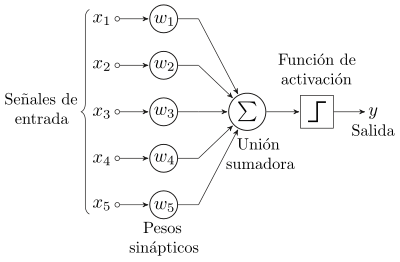
\includegraphics[width=0.5\textwidth]{../img/perceptron}\caption{Diagrama de un perceptrón simple con cinco entradas}
\end{figure}

Conectando entre sí varios de estos perceptrones podríamos comenzar a hablar de redes neuronales.


\section{Algoritmos genéticos}

 Los algoritmos genéticos son una parte de la inteligencia artificial cuyo objetivo es optimizar los resultados intentando emular las leyes de la naturaleza, la evolución natural \cite{AraujoCervigon}. Es un tipo de algoritmo muy eficaz en la mayor parte de problemas dada su gran versatilidad.

La clave de un algoritmo evolutivos reside, como en la naturaleza, en la supervivencia de los mejor adaptados \cite{JHolland}. Para llegar a estos individuos mejor adaptados, siempre se suelen seguir los mismos pasos. Los paso a seguir son inicialización, evaluación, selección, cruce y, opcionalmente, mutación.

Antes de todo este proceso hay que analizar el problema y decidir cuál va a ser su representación, la representación de un individuo. Comúnmente este tipo de problemas se representan en forma de array unidimensional en el que cada posición de éste representará una característica del individuo. Los atributos o características del individuo son valores numéricos que, dependiendo del problema, pueden ser binarios, continuos, discretos, etc. Cuanto mejor se represente el problema, evidentemente, más probable es que consigamos alcanzar un resultado óptimo. 

\begin{figure}[ht]
\begin{minipage}[b]{0.56\linewidth}
\centering
\begin{tabular}{|c|c|c|c|c|c|}
\hline
 0 & 1 & 1 & 0 & 0 & 1 \\ \hline
\end{tabular}
    \caption{Representación del individuo}
    \label{table:individuo}
\end{minipage}\hfill
\begin{minipage}[b]{0.4\linewidth}

\centering
  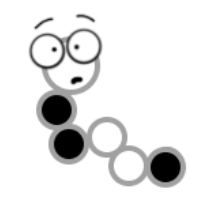
\includegraphics[width=0.5\textwidth]{../img/gusanete}\label{fig:f1}
  \caption{Individuo}
\end{minipage}
\end{figure}
    


\textbf{Inicialización:} Para la inicialización se generan individuos aleatorios, esto es, rellenar con valores aleatorios los arrays que representan a nuestros individuos. Un array define las características de un individuo y un conjunto de individuos define una población. Esta población inicial, partiendo del absoluto azar será previsiblemente mala.

\textbf{Evaluación:} Para estimar la calidad de un undividuo debemos definir una función de \emph{fitness}, es decir, una función que nos de un valor (\emph{fitness}) comparable que nos indique lo bueno o malo que es frente al resto de la población.

\textbf{Selección:} Una vez ya hemos evaluado a todos los individuos se pasa al proceso de selección. En este punto se pueden descartar directamente aquellos individuos que cuyo \emph{fitness} no supere un umbral mínimo definido por nosotros. Pasado este primer corte procedemos a elegir los mejores indivíduos, existen diferentes criterios de selección: selección Proporcional (o Ruleta), muestreo estocástico universal, selección por torneo, etc.

\textbf{Cruce:} Para poder seguir avanzando a lo largo de las generaciones necesitamos generar nuevos individuos. Uno de los operadores encargado de la generación de nuevos individuos es el operador de cruce. El operador de cruce establece una probabilidad determinada de que un individuo sea seleccionado para el cruce, si este supera ese umbral el individuo procederá a cruzarse. El cruce se realiza intercambiando secciones de su genotipo en uno o varios puntos aleatorios. En la figura \ref{cruce_monopunto} tenemos un ejemplo de cruce monopunto \cite{cruce_monopunto}.

\begin{figure}[h]
  \centering
  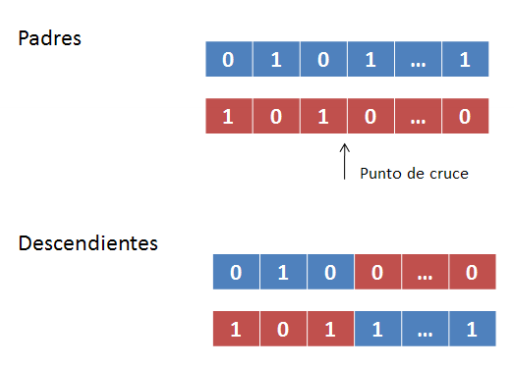
\includegraphics[width=0.5\textwidth]{../img/cruce_monopunto}\caption{Ejemplo de cruce Monopunto}\label{cruce_monopunto}
\end{figure}



\textbf{Mutación:} Otro de los operadores más utilizados en la generación de nuevos individuos es el operador de mutación. Cuando se va a proceder a la mutación se establece una probabilidad de mutación y se va evaluando cada elemento del genotipo, es decir, se saca un número aleatorio y si este supera el umbral de mutación, ese gen resulta mutado. Durante el proceso de mutación pueden surgir individuos peores que sus predecesores, por lo tanto habrá que ser cauto estableciendo el parámetro de mutación.

\textbf{Reemplazo:} Para finalizar, antes de comenzar de nuevo todo este proceso, debemos reemplazar los individuos descartados por lo nuevos para conformar la nueva población. Una vez hecho este reemplazo, se procede de nuevo con todos los pasos. Hay varios criterios de parada, los más comunes suelen ser por convergencia, por tiempo o por número de generaciones.

\imagen{evolutive}{Esquema de algoritmo evolutivo simple}



